\documentclass[
    11pt, % Set the default font size, options include: 8pt, 9pt, 10pt, 11pt, 12pt, 14pt, 17pt, 20pt
%t, % Uncomment to vertically align all slide content to the top of the slide, rather than the default centered
%aspectratio=169, % Uncomment to set the aspect ratio to a 16:9 ratio which matches the aspect ratio of 1080p and 4K screens and projectors
]{beamer}


\usepackage{booktabs} % Allows the use of \toprule, \midrule and \bottomrule for better rules in tables
\usepackage{xcolor}
\usepackage{listings}
\lstset{
    basicstyle=\ttfamily,
    language=make,
    columns=fullflexible,
    breaklines=true,
    showstringspaces=false,
}
\usepackage{hyperref}

%----------------------------------------------------------------------------------------
% LAYOUT THEME
\usetheme{Madrid}
%----------------------------------------------------------------------------------------

%----------------------------------------------------------------------------------------
% COLOR THEME
\usecolortheme{whale}
%----------------------------------------------------------------------------------------

%----------------------------------------------------------------------------------------
% FONT THEME & FONTS
\usefonttheme{serif}
%----------------------------------------------------------------------------------------

%\usepackage{mathptmx} % Use the Times font for serif text
\usepackage{amsmath}
\usepackage{palatino} % Use the Palatino font for serif text
%\usepackage{helvet} % Use the Helvetica font for sans serif text
\usepackage[default]{opensans}
\usepackage{textcomp} % Use the Open Sans font for sans serif text
\usepackage{scrextend}
%\usepackage[default]{FiraSans} % Use the Fira Sans font for sans serif text
%\usepackage[default]{lato} % Use the Lato font for sans serif text



%----------------------------------------------------------------------------------------
% INNER THEME
\useinnertheme{circles}
%----------------------------------------------------------------------------------------

%\setbeamertemplate{footline} % Removes the footer line in all slides
%\setbeamertemplate{footline}[page number] % Replace the footer line in all slides with a simple slide count
%\setbeamertemplate{navigation symbols}{} % Remove the navigation symbols from the bottom of all slides

%----------------------------------------------------------------------------------------
%	PRESENTATION INFORMATION
\title[swc]{Smart Waste Collection \\ Elaborato di progetto per il corso LSS}
\author[Baiardi, Marcantoni, Romagnoli, Spadoni]{Martina Baiardi - Alessandro Marcantoni\\Simone Romagnoli - Marta Spadoni}
\date[14/07/2022]{14/07/2022}
%----------------------------------------------------------------------------------------

\begin{document}

% TITLE SLIDE ----------------------------------------------------------------------------
    \begin{frame}
        \titlepage
    \end{frame}
%----------------------------------------------------------------------------------------

% TABLE OF CONTENTS SLIDE ---------------------------------------------------------------
    \begin{frame}
        \frametitle{Overview}
        \tableofcontents
    \end{frame}
%----------------------------------------------------------------------------------------

    \section{Introduzione}
\frame{\tableofcontents[currentsection]}

%-------------------------------------------------

\begin{frame}
    \frametitle{Obiettivi del progetto}
    L'obiettivo principale del progetto è quello di ottimizzare la gestione della raccolta dei rifiuti utilizzando
    tecnologie innovative.

    \bigskip

    In particolare, si vuole:
    \begin{itemize}
        \item Dotare di sensori i cassonetti e i camioncini dei rifiuti, per poterne monitorare lo stato.
        \item Automatizzare la creazione delle missioni di raccolta, per renderle più efficienti.
        \item Migliorare la gestione dei rifiuti "straordinari", ossia quelli che richiedono una raccolta particolare.
        \item Monitorare lo stato di funzionamento dei servizi offerti dall'organizzazione.
    \end{itemize}

\end{frame}
%------------------------------------------------
    \section{Analisi del Dominio}
\frame{\tableofcontents[currentsection]}

%-------------------------------------------------
\subsection{Analisi del Problema}

\begin{frame}
    \frametitle{Analisi del Problema}
    È stata condotta un'intervista con degli esperti di dominio che hanno consentito di chiarire quale sia l'attuale
    funzionamento del sistema.
    Questi hanno inoltre espresso i miglioramenti che desiderano vengano introdotti nella gestione della raccolta dei
    rifiuti.

    \bigskip

    Grazie alle risposte ottenute è stato possibile costruire un \textbf{Ubiquitous Language} condiviso tra il team di sviluppo
    e l'azienda.

\end{frame}
%------------------------------------------------

%-------------------------------------------------
\subsection{Ubiquitous Language}

\begin{frame}
    \frametitle{Ubiquitous Language}
    Grazie all'appronfondita analisi del dominio che è stata effettuata con i committenti, il team ha prodotto un
    \textbf{Ubiquitous Language}.

    \bigskip

    La costruzione di questo vocabolario ha consentito a tutti i membri del team di avere chiaro quali siano gli
    elementi che sono presenti all'interno del dominio e quali siano i loro ruoli, rimuovendo tutte le ambiguità.

    \bigskip

    L'Ubiquitous Language ha consentito agli sviluppatori di lavorare in modo indipendente e parallelo su componenti
    differenti del sistema.

\end{frame}
%------------------------------------------------

%-------------------------------------------------
\subsection{Analisi dell'Impatto}

\begin{frame}
    \frametitle{Analisi dell'Impatto}
    Per fare chiarezza con l'organizzazione sull'impatto del progetto è stato realizzato un \textbf{Impact Mapping}.

    \smallskip

    \begin{figure}[H]
        \centering
        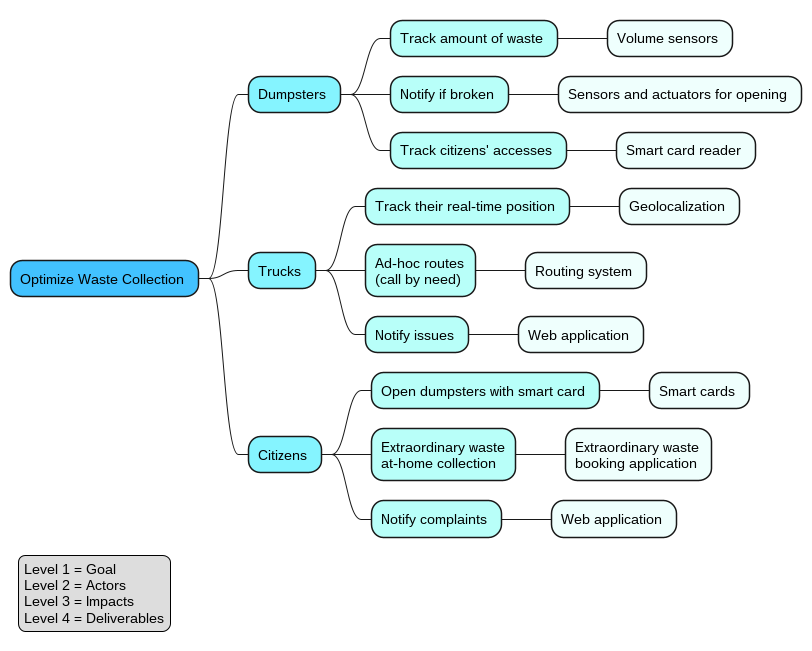
\includegraphics[width=0.7\linewidth]{../img/impact-mapping}
    \end{figure}

\end{frame}
%------------------------------------------------

    \section{Requisiti}
\frame{\tableofcontents[currentsection]}

%-------------------------------------------------
\begin{frame}
    \frametitle{Requisiti}
    Per definire i requisiti del sistema che verrà sviluppato, sono state utilizzate due tecniche:

    \begin{itemize}
        \item \textbf{User Stories}: Per delineare quali sono i requisiti richiesti dal punto di vista degli utilizzatori
        del sistema.
        \item \textbf{Use Cases}: Per una rappresentazione tramite \textit{diagrammi dei casi d'uso} per evidenziare le
        interazioni tra i vari attori del sistema.
    \end{itemize}

\end{frame}
%------------------------------------------------

%-------------------------------------------------
\subsection{User Stories}

\begin{frame}
    \frametitle{User Stories}
    Le \textbf{User Stories} sono state definite dal punto di vista di \textbf{Managers}, \textbf{Citizens} e
    \textbf{Truck Drivers}, seguendo il pattern:

    \bigskip

    \begin{block}{}
        \begin{center}
            \texttt{\textbf{As a} ... \textbf{I want to} ... \textbf{So that} ...}
        \end{center}
    \end{block}

    \bigskip

    Ad esempio:

    \medskip

    \begin{addmargin}[1em]{2em}
        \textit{\textbf{As a} Citizen \textbf{I want to} book an "at home" waste collection \textbf{so that} I don't have to go to the disposal point. }
    \end{addmargin}

\end{frame}
%------------------------------------------------

%-------------------------------------------------
\subsection{Use Cases}

\begin{frame}
    \frametitle{Use Cases}
    Dopo aver analizzato le funzionalità dal punto di vista degli attori del sistema, sono stati definiti dei
    diagrammi UML che ne descrivono i comportamenti.

    \bigskip

    In particolare sono stati evidenziati le seguenti "macro-funzionalità":
    \begin{itemize}
        \item Gestione della raccolta dei \textbf{rifiuti ordinari}
        \item Gestione della raccolta dei \textbf{rifiuti straordinari}
        \item \textbf{Dashboard}
        \item Gestione dei \textbf{reclami}
    \end{itemize}
\end{frame}
%------------------------------------------------

    \section{Design}
\frame{\tableofcontents[currentsection]}

%-------------------------------------------------
\subsection{Design del Dominio}

%-------------------------------------------------
\begin{frame}
    \frametitle{Bounded Contexts}
    Dopo aver effettuato la fase di analisi, il team ha delineato i \textbf{Subdomain} e i \textbf{Bounded Context} che
    compongono il dominio.

    \smallskip

    \begin{figure}[H]
        \centering
        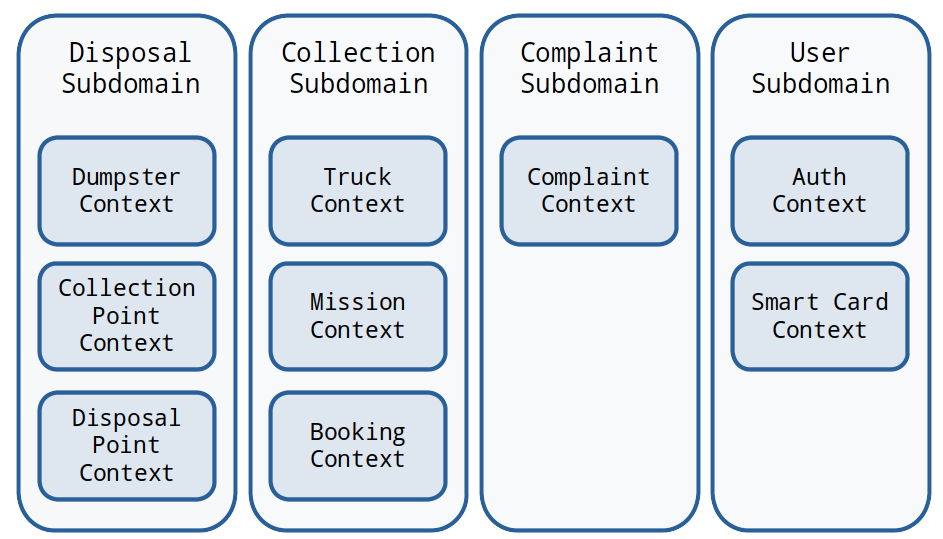
\includegraphics[width=0.8\linewidth]{../img/bounded-contexts}
    \end{figure}

\end{frame}
%------------------------------------------------
%-------------------------------------------------
\begin{frame}
    \frametitle{Context Mapping}
    Una volta individuati i \textbf{Subdomain} sono state analizzate le possibili relazioni che avvengono tra di essi.

    \bigskip

    In particolare, sono state individuate due tipologie di interazione:
    \begin{itemize}
        \item \textbf{Partnership}: dove i componenti si accordano sull'integrazione delle funzionalità
        \item \textbf{Upstream - Downstream (Conformist)}: dove il downstream si adatta alla specifica api definita dall'upstream
    \end{itemize}

\end{frame}
%------------------------------------------------

%-------------------------------------------------
\begin{frame}
    \frametitle{Context Mapping}

    \begin{figure}[H]
        \centering
        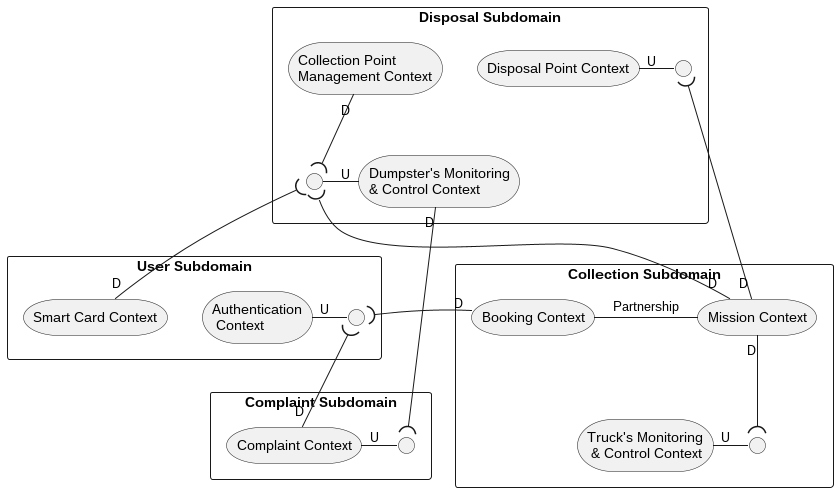
\includegraphics[width=\linewidth]{../img/context-mapping}
    \end{figure}

\end{frame}
%------------------------------------------------
%-------------------------------------------------
\begin{frame}
    \frametitle{Domain Models}
    Sono stati modellati gli elementi \textit{core} del dominio utilizzando i \textbf{Tactical Building Blocks},
    definendo i principali \textbf{Aggregates}.

    \bigskip

    Gli aggregates modellati sono:
    \begin{itemize}
        \item \textbf{Dumpster Aggregate}
        \item \textbf{Collection Point Aggregate}
        \item \textbf{Truck Aggregate}
        \item \textbf{Mission Aggregate}
    \end{itemize}

    \bigskip

    All'interno di ciascuno di essi sono stati specificati: \textit{Entities}, \textit{Value Objects},
    \textit{Domain Services} e \textit{Domain Events}.

\end{frame}
%------------------------------------------------

%-------------------------------------------------
\begin{frame}
    \frametitle{Context Mapping}

    \begin{figure}[H]
        \centering
        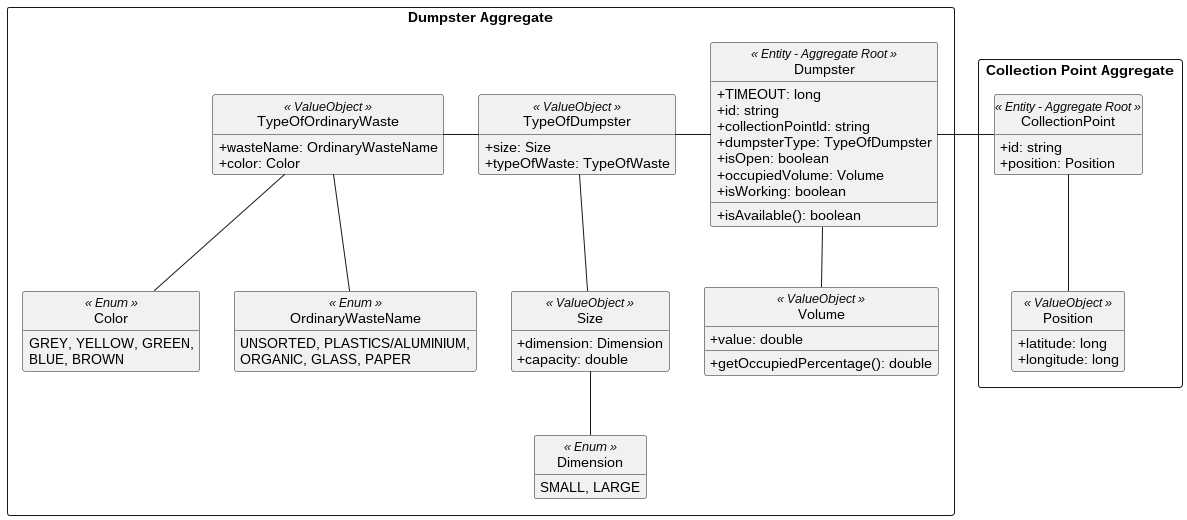
\includegraphics[width=\linewidth]{../img/disposal-domain-model}
    \end{figure}

\end{frame}
%------------------------------------------------
%------------------------------------------------

%-------------------------------------------------
\subsection{Design Architetturale}

%-------------------------------------------------
\begin{frame}
    \frametitle{Architettura}
    È stata definita una architettura ad alto livello del sistema, a partire dai \textbf{Subdomain} precedentemente
    identificati.

    \bigskip

    Per ciascuno di essi, vengono individuati i \textit{microservizi} necessari per il funzionamento del sistema,
    specificando anche le interazioni che avvengono tra essi.

    \smallskip

    \begin{figure}[H]
        \centering
        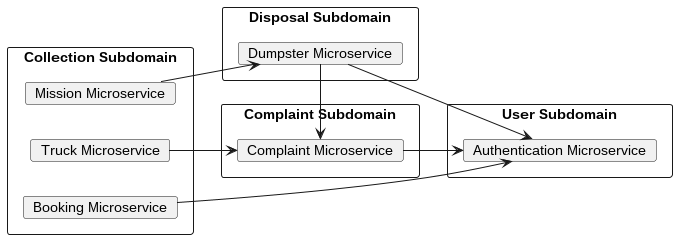
\includegraphics[width=0.8\linewidth]{../img/global-architectural-map}
    \end{figure}

\end{frame}
%------------------------------------------------

%-------------------------------------------------
\begin{frame}
    \frametitle{Architettura dei Microservizi}
    Ciascun microservizio è stato implementato ispirandosi alla \textbf{Clean Architecture}.

    \smallskip

    \begin{columns}
        \begin{column}{0.6\textwidth}
            In particolare, sono state definiti i seguenti layer:
            \begin{itemize}
                \item \textbf{Entities}
                \item \textbf{Use Cases}
                \item \textbf{Adapters}
                \item \textbf{Drivers}
            \end{itemize}
        \end{column}
        \begin{column}{0.4\textwidth}
            \begin{center}
                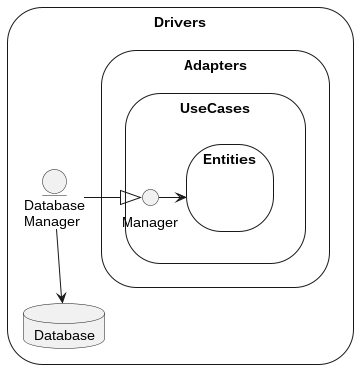
\includegraphics[width=\textwidth]{../img/clean}
            \end{center}
        \end{column}
    \end{columns}


\end{frame}
%------------------------------------------------

%------------------------------------------------


    \section{Devops}
\frame{\tableofcontents[currentsection]}

%-------------------------------------------------
\subsection{DVCS Strategy}
\begin{frame}
    \frametitle{DVCS Strategy}
    Per gestire i repository sono state effettuate le seguenti scelte:
    \begin{itemize}
        \item Definizione di una \textbf{GitHub Organization} per contenere tutti i progetti.
        \item Utilizzo di \textbf{Git Flow Workflow} per avere una linea di sviluppo chiara e ben definita.
        \item Utilizzo dei \textbf{Conventional Commit} per poter generare in modo automatico i nuovi \textbf{tag} e le relative \textbf{release}
        \item Configurazione di un \textbf{Commit Linter} per assicurare che i commit siano correttamente formattati
    \end{itemize}
\end{frame}
%------------------------------------------------

%-------------------------------------------------
\subsection{Continuous Integration}
\begin{frame}
    \frametitle{Continuous Integration}
    All'interno dei repository dell'organizzazione sono stati configurati dei workflow che, tramite delle GitHub Actions,
    effettuano i seguenti controlli:
    \begin{itemize}
        \item \textbf{Code Quality Control}: tramite i plugin \texttt{ktlint} e \texttt{ESLint}.
        \item \textbf{Testing}: utilizzando i plugin \texttt{kotest} e \texttt{mocha}.
        \item \textbf{Reporting della coverage}: con i plugin \texttt{jacoco} e \texttt{istanbul}.
    \end{itemize}

    \bigskip

    Inoltre è stato configurato il bot \texttt{renovate} all'interno dei repository per effettuare \textbf{Automatic Dependency Update}.

\end{frame}

%------------------------------------------------

%-------------------------------------------------
\subsection{Continuous Delivery}
\begin{frame}
    \frametitle{Continuous Delivery}
    Sono stati inoltre configurati dei workflow che consentono di effettuare:
    \begin{itemize}
        \item \textbf{Semantic Versioning and Releasing}: GitHub Action che consente di calcolare automaticamente il tag della release ed effettuarla tramite l'analisi dei messaggi di commit.
        \item \textbf{Containerization}: L'applicazione viene costruita utilizzando un Dockerfile e pubblicata all'interno dei GitHub Packages.
    \end{itemize}
\end{frame}


%------------------------------------------------



\end{document}
